
\documentclass[nototal]{beamer}
\mode<presentation>
{
  \usetheme{Madrid}
  \setbeamercovered{transparent}
}

\usepackage{verbatim}
\usepackage{fancyvrb}
\usepackage[english]{babel}
\usepackage[latin1]{inputenc}
\usepackage{times}
\usepackage{tikz}
\usepackage[T1]{fontenc}
\usepackage{graphicx} %sjr added
\graphicspath{{figures/}}
\usepackage{hyperref}

\author{\textsc{Sergio Rey}}
\institute[ASU]{\textbf{GPH 483/598}\\\textbf{Geographic Information
Analysis}\\School of Geographical Sciences\\Arizona State University\\Spring
2010}
\title[GPH 483/598]{Point Pattern Analysis: Basics}
\subtitle{}
\date[Point Patterns Basics]{}

% Delete this, if you do not want the table of contents to pop up at
% the beginning of each subsection:
\AtBeginSubsection[]
{
  \begin{frame}<beamer>
    \frametitle{Outline}
    \tableofcontents[currentsection,currentsubsection]
  \end{frame}
}


% If you wish to uncover everything in a step-wise fashion, uncomment
% the following command: 
\beamerdefaultoverlayspecification{<+->}
\begin{document}
\begin{frame}
  \titlepage
\end{frame}
\begin{frame}
  \frametitle{Outline}
  \tableofcontents[pausesections]
  % You might wish to add the option [pausesections]
\end{frame}

\section{Point Pattern Analysis Objectives and Examples}
\subsection{Objectives}
\begin{frame}[<+->]
  \frametitle{Point Pattern Analysis Objectives}
  \begin{block}{Goals}
    \begin{itemize}
      \item Pattern detection
      \item Assessing the presence of  \emph{clustering}
      \item Identification of individual \emph{clusters}
    \end{itemize}
   \end{block}
\begin{block}{General Approaches}
    \begin{itemize}
      \item Estimate intensity of the process
      \item Formulating an idealized model and investigating deviations from
	expectations 
      \item Formulating  a stochastic model and fitting it to the data
    \end{itemize}
   \end{block}
 \end{frame}

\subsection{Definitions}
\begin{frame}[<+->]
  \frametitle{Point Pattern Analysis Definitions}
  \begin{block}{Spatial Point Pattern}
    A set of events, irregularly distributed within a region $A$ and presumed
    to have been generated by some form of stochastic mechanism. 
   \end{block}
   \begin{block}{Representation}
$\left\{Y(A),
    A \subset \Re \right\}$, where $Y(A)$ is the number of events occurring in
    area $A$.
   \end{block}
   \begin{block}{Events, points, locations}
     \begin{description}
       \item[Event] an occurrence of interest
       \item[Point] any location in study area
       \item[Event location] a particular point where an event occurs
     \end{description}
\end{block}
\end{frame}

\begin{frame}[<+->]
  \frametitle{Point Pattern Analysis Definitions}
\begin{block}{Region: $A$}
    \begin{itemize}
      \item Most often planar (two-dimensional Euclidean space)
      \item One dimensional applications also possible
      \item Three-dimensional increasingly popular (space + time)
      \item Point processes on networks (non-planar)
    \end{itemize}
   \end{block}
 \end{frame}


\begin{frame}[<+->]
  \frametitle{Space-Time Point Patterns}
    \begin{center}
      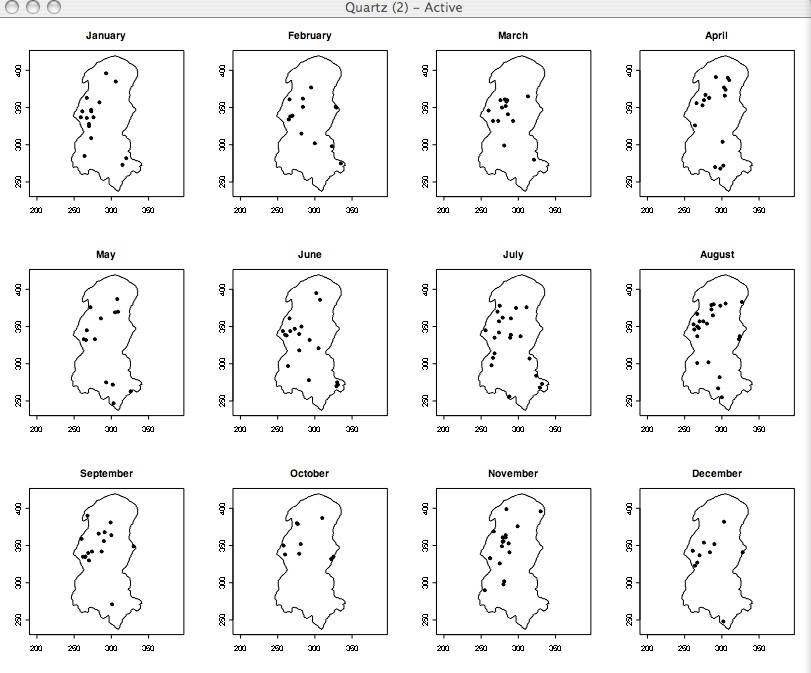
\includegraphics[width=0.65\linewidth]{tspoints}
    \end{center}
  \end{frame}


\begin{frame}[<+->]
    \frametitle{Space-Time Point Patterns}
    \begin{center}
      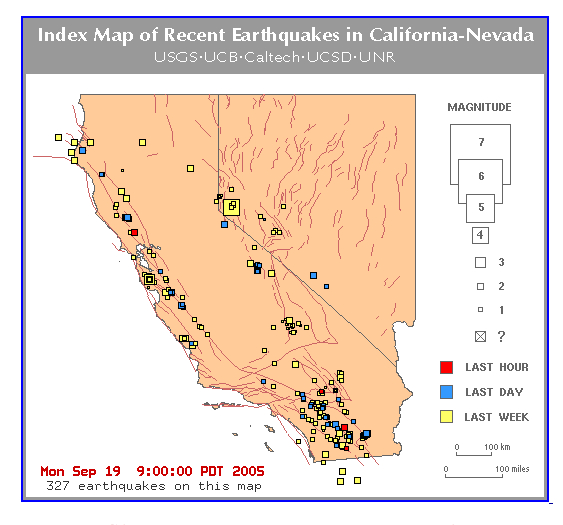
\includegraphics[width=.75\linewidth]{earthquakes.jpg}
    \end{center}
  \end{frame}



\begin{frame}[<+->]
    \frametitle{Point Patterns on Networks}
    \begin{center}
      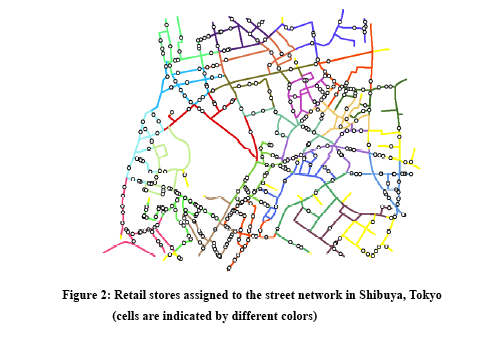
\includegraphics[width=.95\linewidth]{sanet.jpg}
    \end{center}
  \end{frame}
\begin{frame}[<+->]
  \frametitle{Point Patterns}
  \begin{block}{Unmarked Point Patterns}
    \begin{itemize}
      \item Only location is recorded
      \item Attribute is binary (presence, absence)
    \end{itemize}
   \end{block}
\begin{block}{Marked Point Patterns}
    \begin{itemize}
      \item Location is recorded
      \item Non-binary stochastic attribute
      \item e.g., sales at a retail store, dbh of tree
    \end{itemize}
   \end{block}
 \end{frame}

\begin{frame}[<+->]
   \frametitle{Realizations}
\begin{block}{Mapped Point Patterns}
    \begin{itemize}
      \item \emph{All} events are recorded and mapped
      \item Complete enumeration of events
      \item Full information on the realization from the process
    \end{itemize}
   \end{block}
 \begin{block}{Sampled Point Patterns}
    \begin{itemize}
      \item \emph{Sample} of events are recorded and mapped
      \item Complete enumeration of events impossible or intractable
      \item Partial information on the realization from the process
      \item Presence/``absence'' data (ecology, forestry)
    \end{itemize}
   \end{block}

 \end{frame}

\subsection{Examples and Terminology}

\begin{frame}
  \frametitle{Points as Events}
  \begin{block}{Mapped Patterns}
     not a sample
   \end{block}
  \begin{block}{Selection Bias}
    \begin{itemize}
      \item events are mapped
	\item but non-events are not
    \end{itemize}
   \end{block}

 \end{frame}

 \begin{frame}
   \frametitle{Research Questions}
   \begin{block}{Location Only}
      are points randomly located or patterned
    \end{block}
   \begin{block}{Location and Value}
     \begin{itemize}
       \item marked point pattern
       \item is combination of location and value random or patterned
     \end{itemize}
    \end{block}
   \begin{block}{Both Cases}
    What is the Underlying Process?
    \end{block}
  \end{frame}

  \begin{frame}
    \frametitle{Points on a Plane}
    \begin{block}{Classic Point Pattern Analysis}
      \begin{itemize}
	\item points on an isotropic plane
	\item no effect of translation and rotation
	\item classic examples: tree seedlings, rocks, etc
      \end{itemize}
     \end{block}
     \begin{block}{Distance}
       \begin{itemize}
	 \item no directional effects
	 \item no translational effects
	  \item straight line distance only
       \end{itemize}
     \end{block}
   \end{frame}


\begin{frame}
     \frametitle{Events: Point Map}
     % maybe fire data?
     \begin{center}
       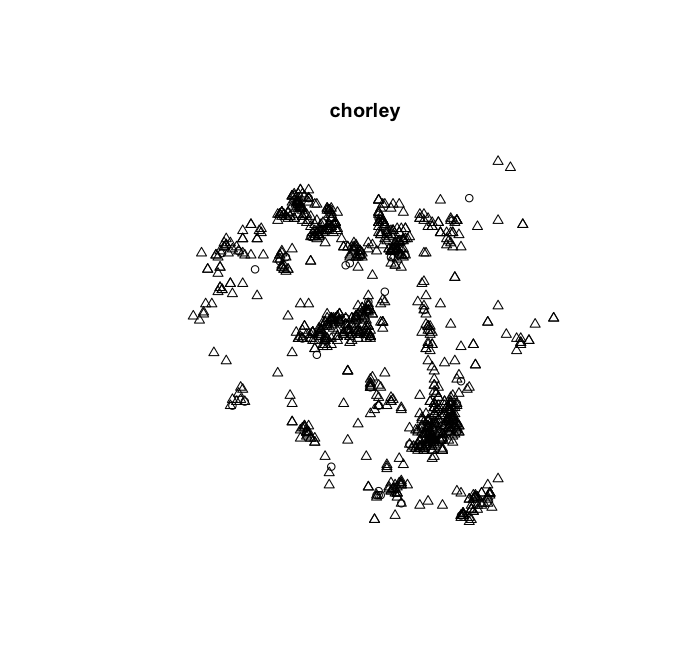
\includegraphics[width=.65\linewidth]{chorley.png}
     \end{center}
   \end{frame}

\begin{frame}
     \frametitle{Points in Context}
     % maybe fire data?
     \begin{center}
       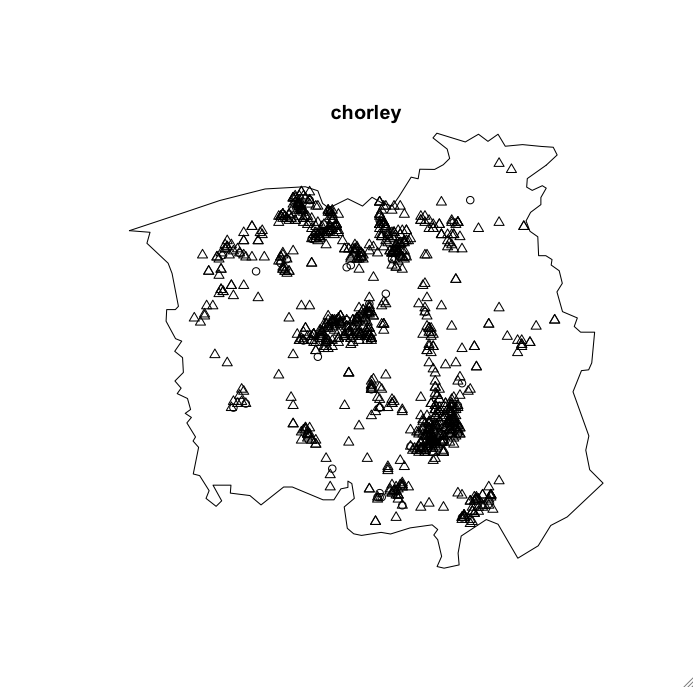
\includegraphics[width=.65\linewidth]{chorleypoly.png}
     \end{center}
   \end{frame}

   \begin{frame}
     \frametitle{Intensity}
     \begin{block}{First Moment}
       \begin{itemize}
	 \item number of points $N$, area of study $|A|$
	 \item intensity: $\lambda = N/|A|$
	 \item area depends on bounds, often arbitrary
       \end{itemize}
      \end{block}
     \begin{block}{Artificial Boundaries}
       \begin{itemize}
	 \item bounding box (rectangle, square)
	 \item other (city boundary)
       \end{itemize}
      \end{block}
    \end{frame}

    % repeat plots w and wo boundary


    \begin{frame}
      \frametitle{Bounding Box}
      \begin{center}
	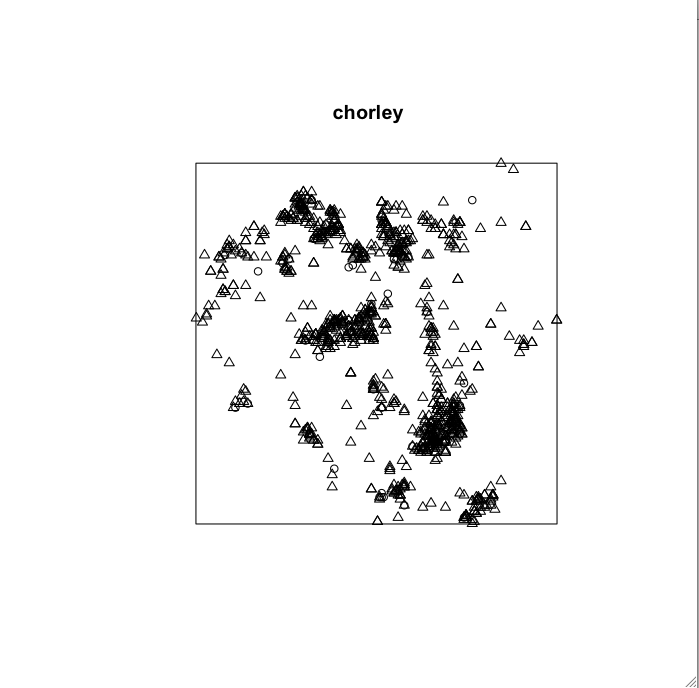
\includegraphics[width=.65\linewidth]{chorleybb.png}
      \end{center}
    \end{frame}

    \begin{frame}
      \frametitle{District Boundary}
      \begin{center}
	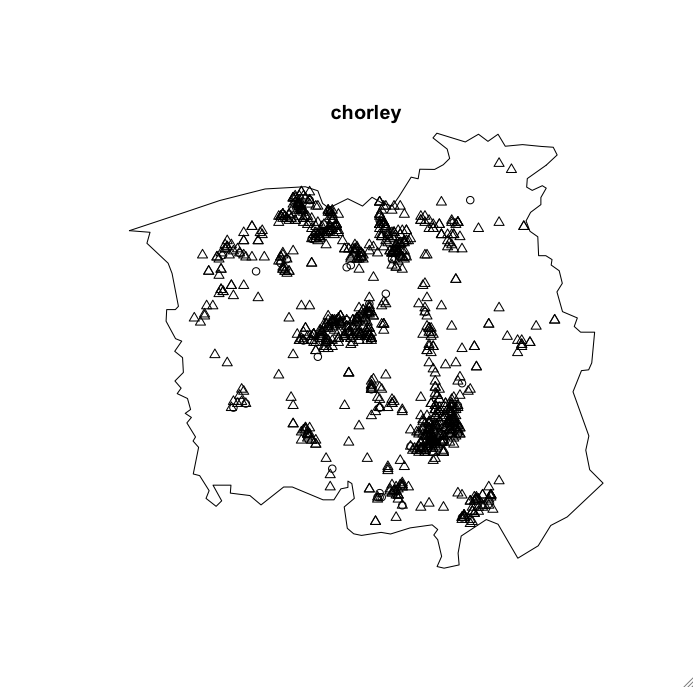
\includegraphics[width=.65\linewidth]{chorleypoly.png}
      \end{center}
    \end{frame}

    \begin{frame}
      \frametitle{Convex Hull}
      \begin{block}{Tightest fit}
	 various algorithms
       \end{block}
       \begin{block}{Rescaled Convex Hull (Ripley-Rasson)}
	\begin{itemize}
	  \item adjust to properly reflect spatial domain of point process
	  \item use centroid of convex hull
	  \item rescale by $1/[\sqrt{(1-m/N)}]$
	  \item $m$: number of vertices of convex hull
	\end{itemize}
       \end{block}
     \end{frame}

     % original convex hull

    \begin{frame}
      \frametitle{Convex Hull}
      \begin{center}
	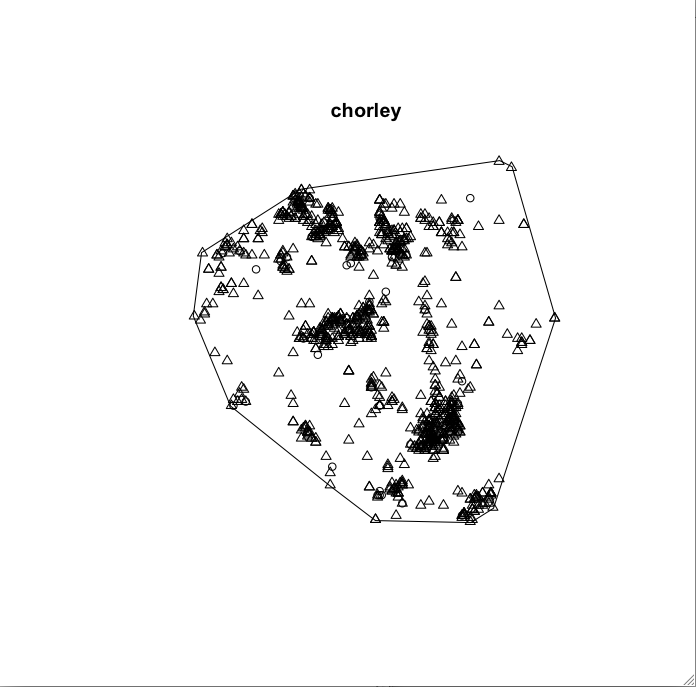
\includegraphics[width=.65\linewidth]{chorleyhull.png}
      \end{center}
    \end{frame}

    \begin{frame}
      \frametitle{Multiple Boundaries}
      \begin{center}
	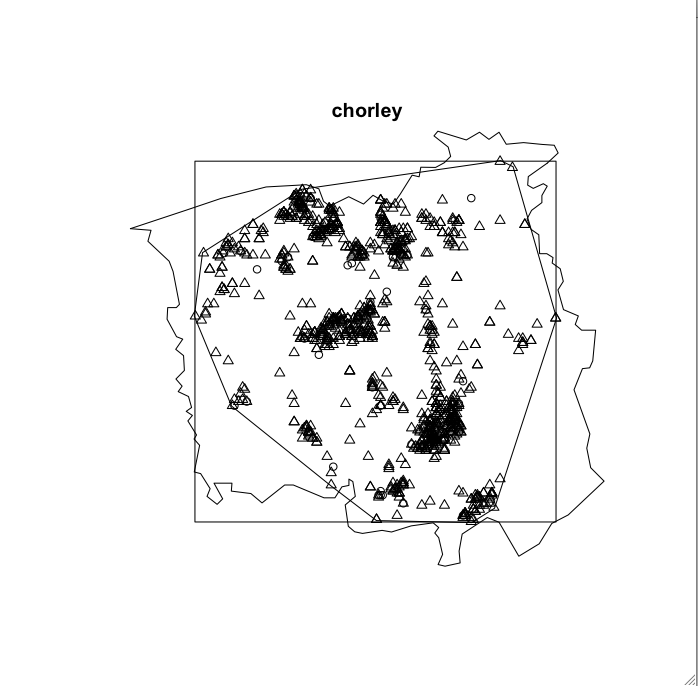
\includegraphics[width=.65\linewidth]{chorleyall.png}
      \end{center}
    \end{frame}


     \begin{frame}
       \frametitle{Intensity Estimates}
       \begin{center}
       \begin{tabular}[h]{lrr}
       & Area& Intensity\\
       & $km^2$& $cases/km^2$\\
       \hline
       District Boundary& 315.155& 3.29\\
       Bounding Box&310.951 &3.33\\
       Convex Hull&229.421 &4.52\\
       \hline
       \end{tabular}\\

       \vspace{0.5in}
       N=1036
     \end{center}
      \end{frame}

      \begin{frame}
	\frametitle{Points on a Network}
	\begin{block}{Realistic Location}
	  \begin{itemize}
	    \item addresses
	    \item remove impossible locations (lakes)
	  \end{itemize}
	 \end{block}
       \begin{block}{Network Distance}
	  \begin{itemize}
	    \item shortest path along network
	    \item Manhattan block distance
	    \item distance vs. travel time or cost
	  \end{itemize}
	 \end{block}
	\end{frame}


	 \begin{frame}
	   \frametitle{Case-Control Design: Lancashire Cancer}
	   \begin{center}
	     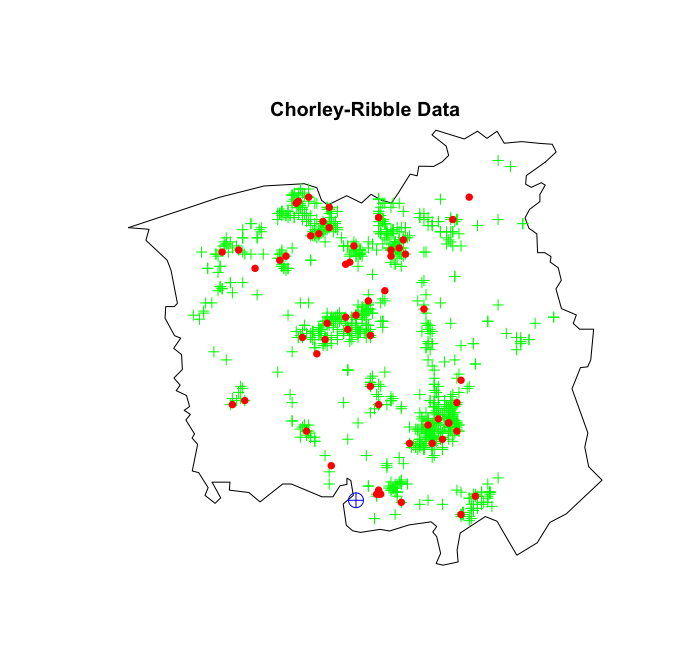
\includegraphics[width=.65\linewidth]{chorleyincin.png}
	   \end{center}
	 \end{frame}

	 \begin{frame}
	   \frametitle{Marked Point Patterns}
	   \begin{block}{Both Location and Value}
	     \begin{itemize}
	       \item Patterns in the Location
	       \item Value Associated with Location
	     \end{itemize}
	    \end{block}
	  \end{frame}

	 \begin{frame}
	   \frametitle{Marked Point Pattern: Longleaf Pine}
	   \begin{center}
	     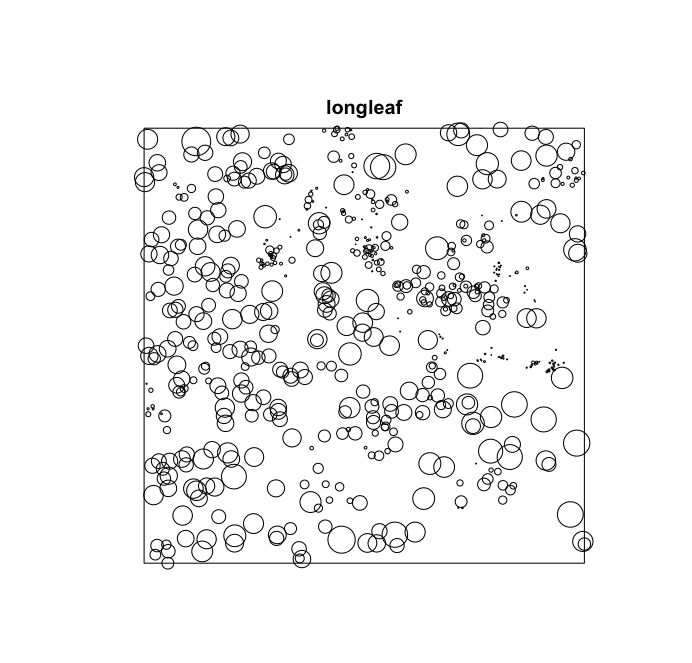
\includegraphics[width=.65\linewidth]{longleaf.png}
	   \end{center}
	 \end{frame}

	 \begin{frame}
	   \frametitle{Multi-Type Patterns}
	   \begin{block}{Multiple Categories}
	     \begin{itemize}
	       \item Patterns in Single Category
	       \item Association between Patterns in Other Categories
	       \item Repulsion or Attraction
	     \end{itemize}
	    \end{block}
	  \end{frame}

	 \begin{frame}
	   \frametitle{Multi-Type Pattern: Lansing Woods}
	   \begin{center}
	     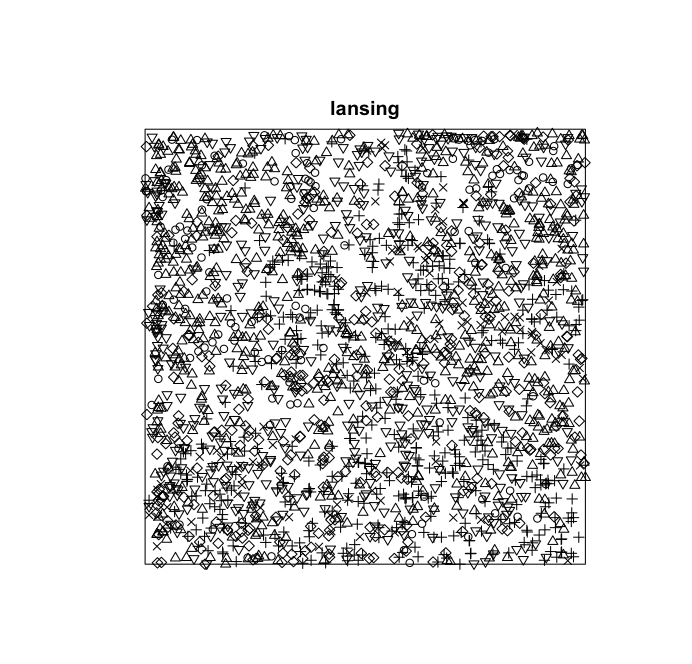
\includegraphics[width=.65\linewidth]{lansing.png}
	   \end{center}
	 \end{frame}

	 \begin{frame}
	   \frametitle{Multi-Type Pattern: Lansing Woods}
	   \begin{center}
	     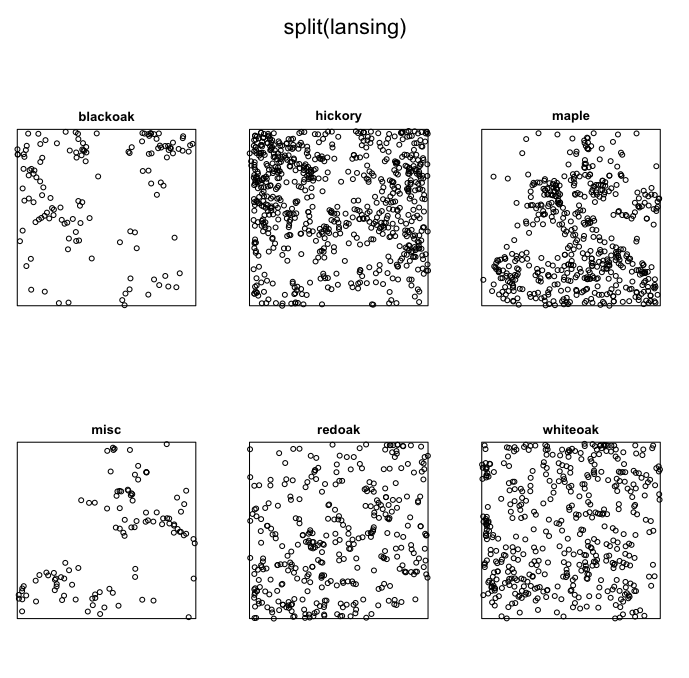
\includegraphics[width=.65\linewidth]{lansingSplit.png}
	   \end{center}
	 \end{frame}


	 \begin{frame}
	   \frametitle{Areal Aggregation}
	   \begin{block}{Event Counts}
	     \begin{itemize}
	       \item points aggregated by areal unit
	       \item spatially extensive variable
	     \end{itemize}
	    \end{block}
	    \begin{block}{Rates}
	      \begin{itemize}
		\item events / population at risk
		\item non-homogeneous population at risk
		\item risk = probability of an event
		\item rate is an estimate of underlying risk
	      \end{itemize}
	    \end{block}
	  \end{frame}

	  \begin{frame}
	    \frametitle{Homicide Counts by Census Tracts}
	    \begin{center}
	      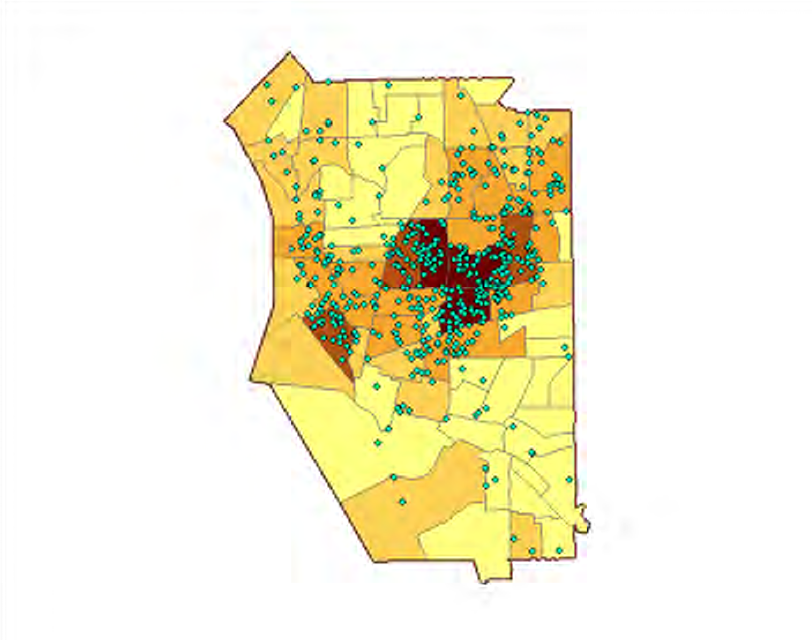
\includegraphics[width=.65\linewidth]{homocideCounts.png}
	    \end{center}
	  \end{frame}

	  \begin{frame}
	    \frametitle{Population Count by Census Tracts}
	    \begin{center}
	      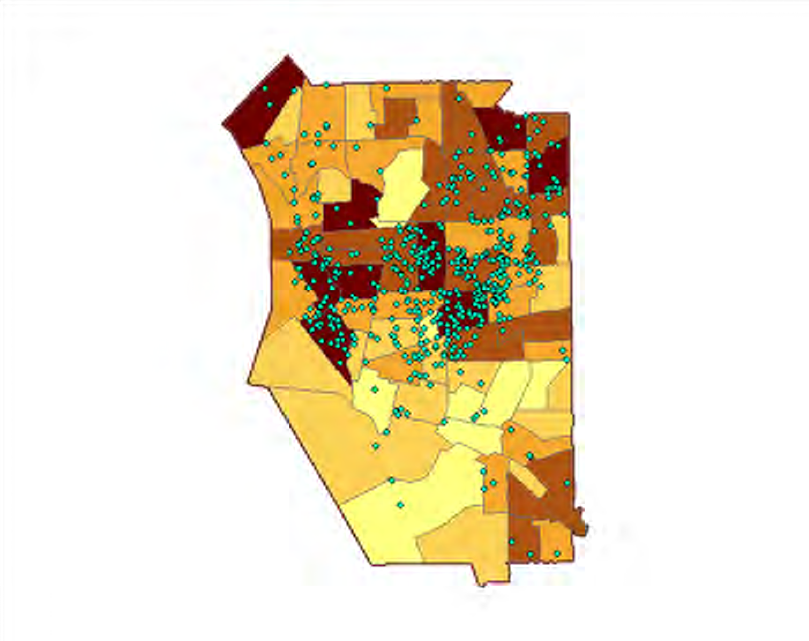
\includegraphics[width=.65\linewidth]{populationCounts.png}
	    \end{center}
	  \end{frame}

	  \begin{frame}
	    \frametitle{Homicide Rate by Census Tracts}
	    \begin{center}
	      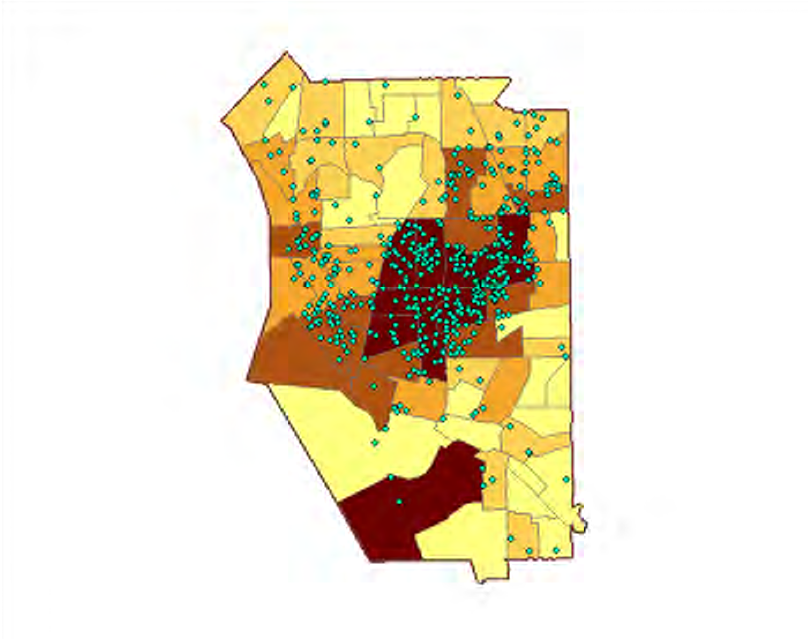
\includegraphics[width=.65\linewidth]{homocideRates.png}
	    \end{center}
	  \end{frame}

\section{Centrography}

\subsection{Central Tendency}
\begin{frame}
  \frametitle{Central Tendency}
  \begin{block}{Purpose}
    \begin{itemize}
      \item Provide a ``center point''
      \item Similar to first moment of a distribution
      \item ``Representative point''
    \end{itemize}
   \end{block}
  \begin{block}{Measures}
    \begin{itemize}
      \item Mean Center
      \item Weighted Mean Center
      \item Median Center
      \item Center of Minimum Distance
    \end{itemize}
   \end{block}
 \end{frame}
 \begin{frame}
   \frametitle{Example Data}
   \begin{center}
   \begin{tabular}[h]{rrrr}
 $i$  &  $x_i$ & $y_i$ &  $w_i$ \\ \hline
1& 20& 40&  10\\
2& 30& 60&  20\\
3& 34& 52&  10\\
4& 40& 40&  20\\
5& 44& 42&  10\\
6& 48& 62&  80\\
7& 50& 10&  10\\
8& 60& 50&  90\\
9& 90& 90& 100\\
  \hline  
   \end{tabular}
 \end{center}
  \end{frame}
 \begin{frame}
   \frametitle{Mean Center}
   \begin{block}{($x_m,y_m$)}
     \begin{equation}
       x_m = 1/n \sum_{i=1}^n x_i
     \end{equation}
     \begin{equation}
       y_m = 1/n \sum_{i=1}^n y_i
     \end{equation}
    \end{block}
  \end{frame}
\begin{frame}
   \frametitle{Mean Center}
   \begin{center}
     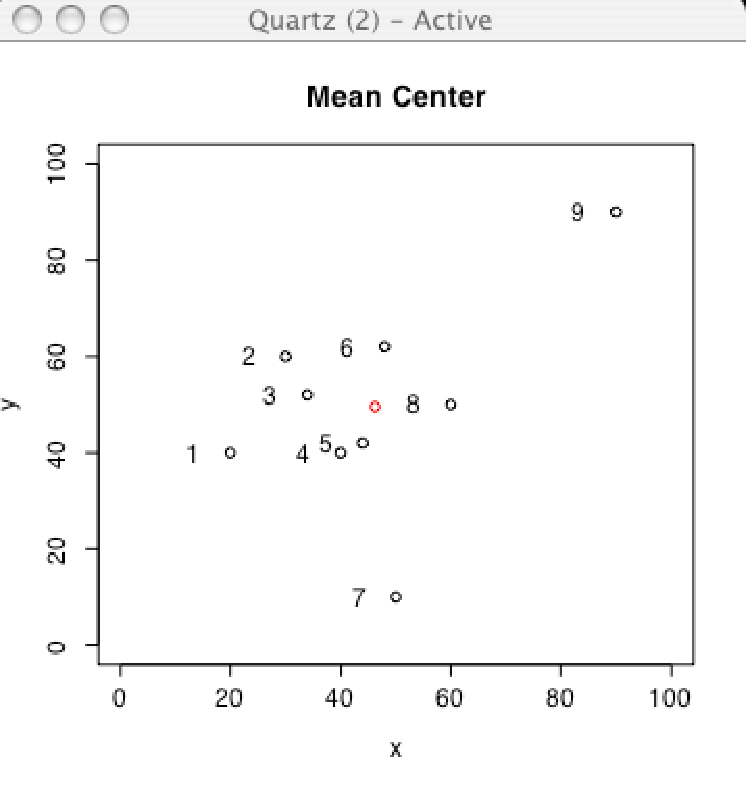
\includegraphics[width=.65\linewidth]{meancenter}
   \end{center}
 \end{frame}


 \begin{frame}
   \frametitle{Weighted Mean center}
   \begin{block}{($x_m,y_m$)}
     \begin{equation}
       x_m = 1/n \sum_{i=1}^n  x_i \frac{w_i}{\sum_{i=1}^n w_i}
     \end{equation}
     \begin{equation}
       y_m = 1/n \sum_{i=1}^n  y_i \frac{w_i}{\sum_{i=1}^n w_i}
     \end{equation}
    \end{block}
    \begin{block}{$w_i$ weight}
      \begin{itemize}
	\item Marked point patterns
	\item Continuous mark
	\item Not categorical mark
      \end{itemize}
    \end{block}
  \end{frame}

\begin{frame}
   \frametitle{Weighted Mean Center}
   \begin{center}
     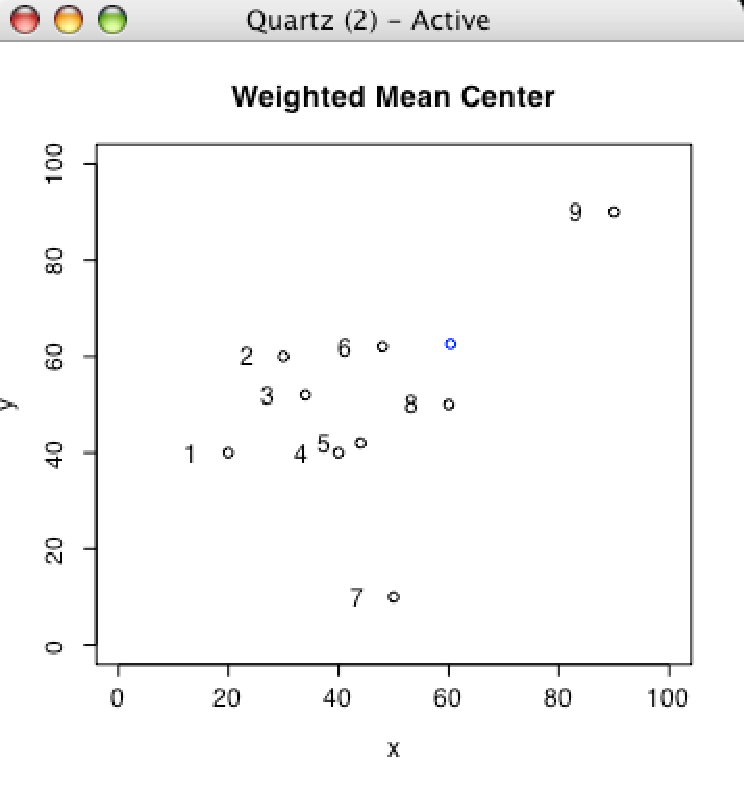
\includegraphics[width=.65\linewidth]{weightedmeancenter}
   \end{center}
 \end{frame}



  \begin{frame}
    \frametitle{Median Center}
    \begin{block}{Definition(s)}
      \begin{description}
	\item[English Statistics] The intersection of two orthogonal axes,
	  each which has an equal number of points on either side.
	\item[American] The center of minimum travel.
      \end{description}
     \end{block}
   \end{frame}

  \begin{frame}
    \frametitle{English Median Center}
    \begin{block}{Manhattan Median}
      \begin{equation}
	Min\ f(x_m,y_m)= \sum_{i=1}^n |x_i - x_m| + |y_i - y_m|
      \end{equation}

     \end{block}
\begin{block}{Advantages}
      \begin{itemize}
	\item Can be found very quickly
	\item No calculations are typically required (other than intersection)
      \end{itemize}
     \end{block}

\begin{block}{Disadvantage}
  \begin{itemize}
    \item Never unique with even $n$
    \item Always unique with odd $n$
    \item Not unique under axis rotation
  \end{itemize}
     \end{block}
   \end{frame}

\begin{frame}
   \frametitle{Manhattan Median}
   \begin{center}
     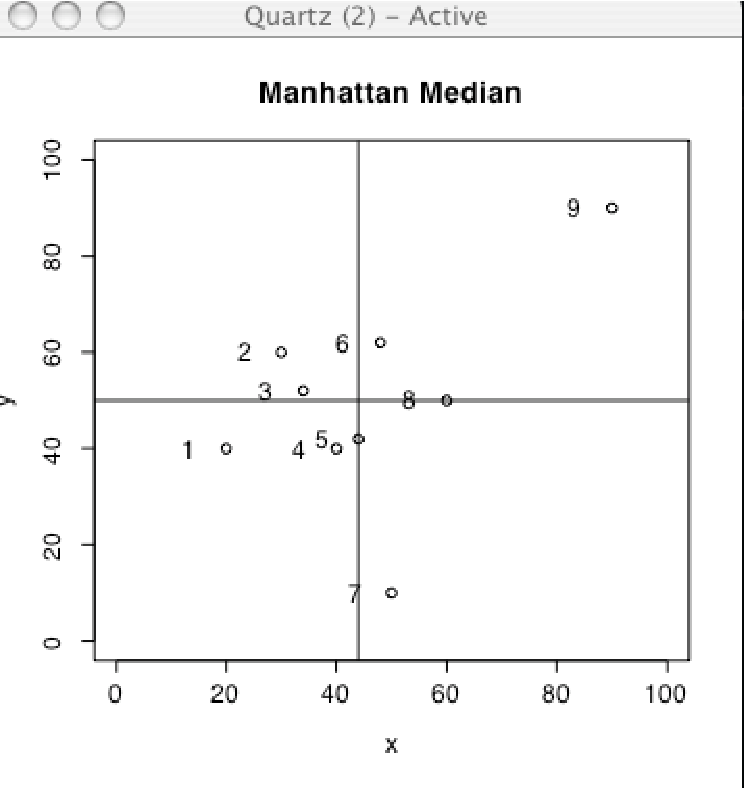
\includegraphics[width=.65\linewidth]{manhattan}
   \end{center}
 \end{frame}

\begin{frame}
   \frametitle{Non-Uniqueness}
   \begin{center}
     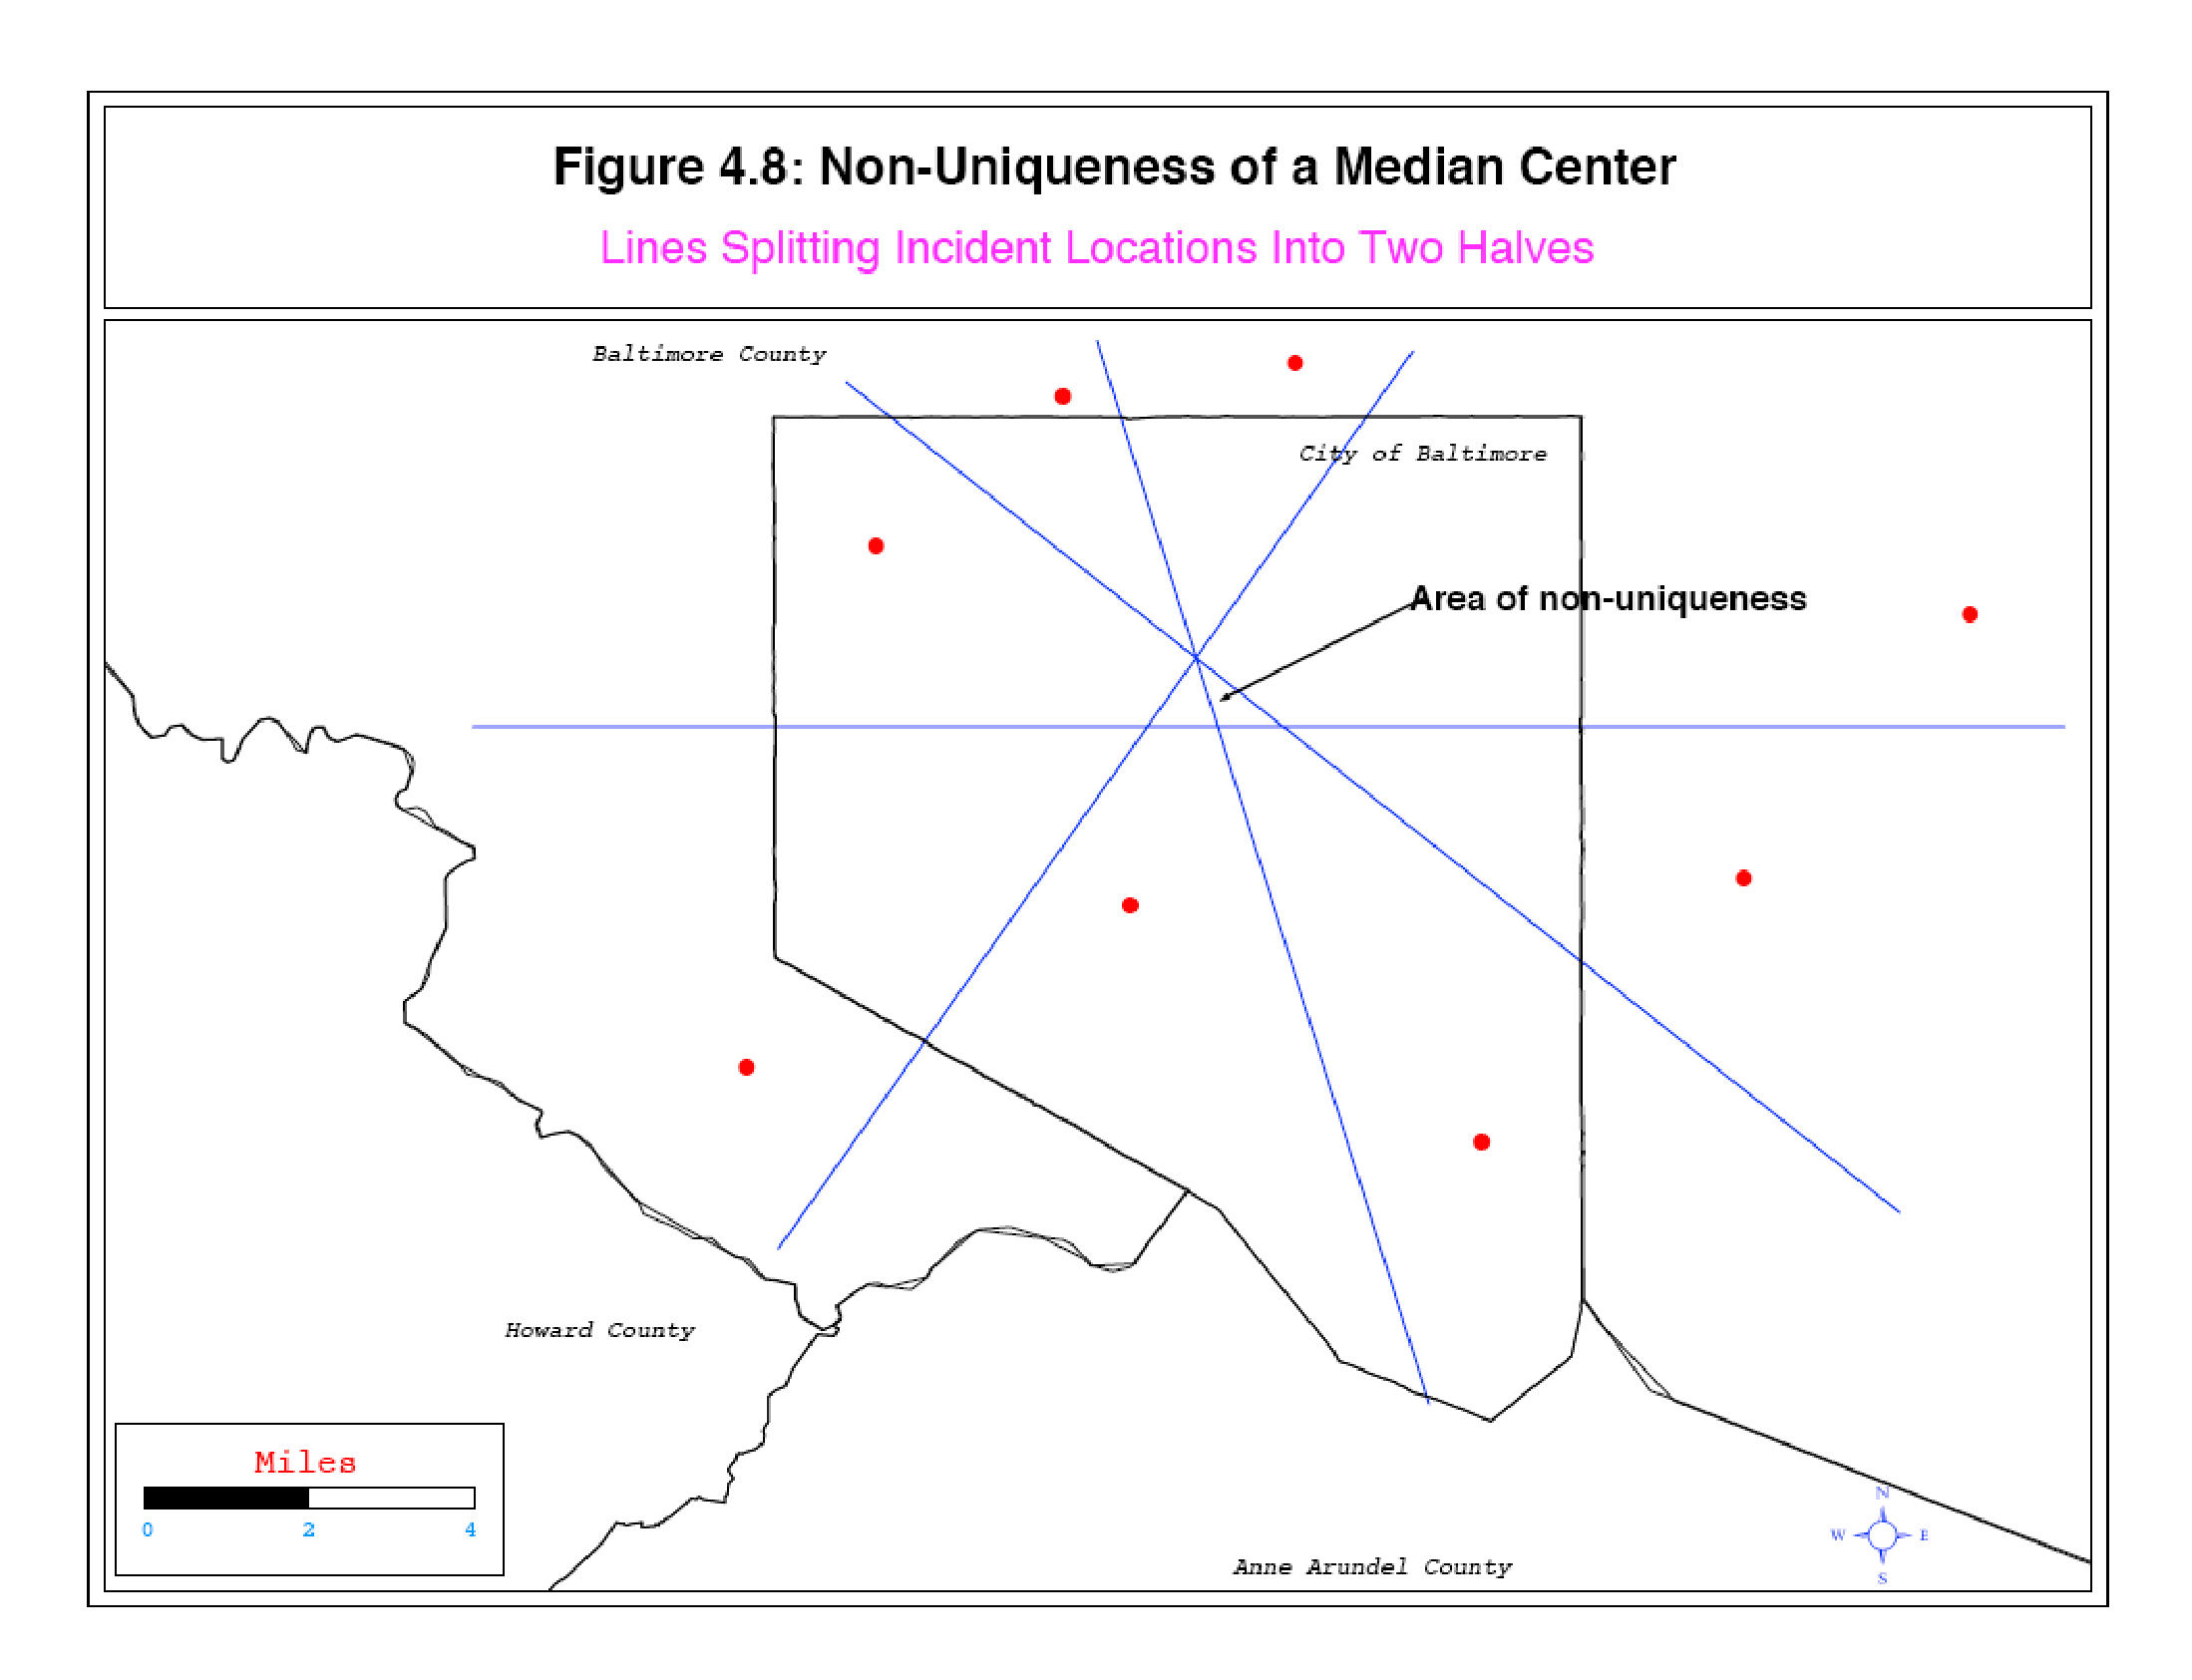
\includegraphics[width=.85\linewidth]{mediancenter1}
   \end{center}
 \end{frame}


  \begin{frame}
    \frametitle{Center of Minimum Travel}
    \begin{block}{Euclidean Median}
      The location from which the sum of the Euclidean distances to all points in a
      distribution is a minimum.
     \end{block}
     \begin{block}{Euclidean Median}
     \begin{equation}
       Min\ f(x_m,y_m)= \sum_{i=1}^n \sqrt{(x_i - x_m)^2 + (y_i - y_m)^2}
      \end{equation}
    \end{block}
      \begin{block}{Weighted Euclidean Median}
     \begin{equation}
       Min\ f(x_m,y_m)= \sum_{i=1}^n\frac{w_i}{\sum_{i=1}^n w_i}
 \sqrt{(x_i - x_m)^2 + (y_i - y_m)^2}
      \end{equation}
    \end{block}

   \end{frame}

   \begin{frame}
     \frametitle{Euclidean Median}
     \begin{block}{Weber Problem}
        Find the optimal location for a factory: one that minimizes transport
	costs between sources of raw materials and delivery to the market.
      \end{block}
     \begin{block}{Solutions}
       \begin{itemize}
	 \item No closed form solution
	 \item First iterative alogrithm: Kuhn and Kuenne (1962)
	 \item Important for more general location allocation problems
       \end{itemize}

     \end{block}
    \end{frame}


\begin{frame}
   \frametitle{Euclidean Median}
   \begin{center}
     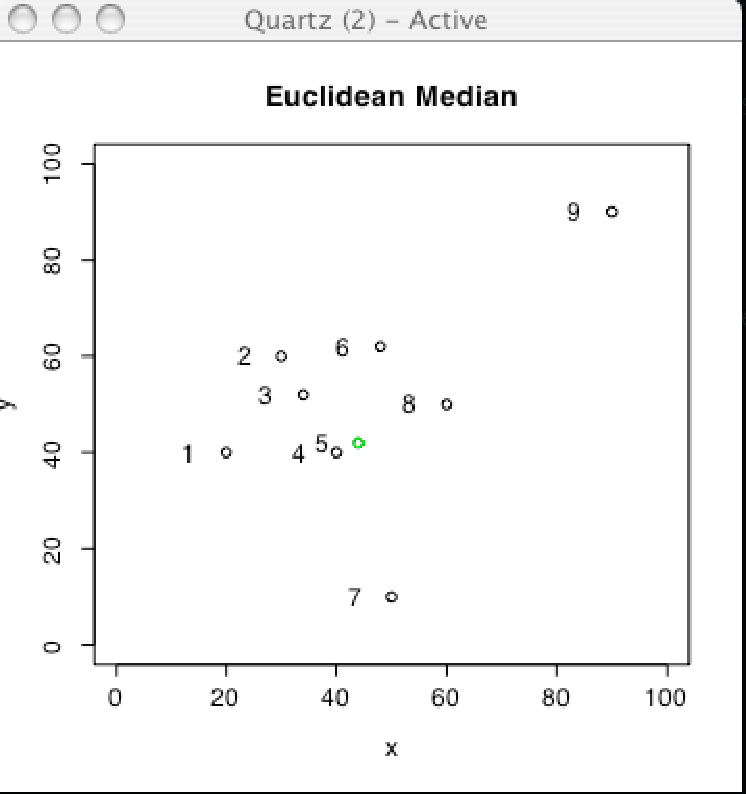
\includegraphics[width=.65\linewidth]{euclideancenter}
   \end{center}
 \end{frame}



\subsection{Dispersion and Orientation}
\begin{frame}
  \frametitle{Dispersion and Orientation}
  \begin{block}{Measures}
    \begin{itemize}
      \item Standard Distance
      \item Major/minor axes
      \item Standard Deviational Ellipse
    \end{itemize}
   \end{block}
 \end{frame}

 \begin{frame}
   \frametitle{Standard Distance}
   \begin{block}{Euclidean Based}
     \begin{equation}
       SD = \sqrt{\frac{\sum_{i=1}^n (x_i-x_m)^2}{n} +\frac{\sum_{i=1}^n (y_i-y_m)^2}{n} }
     \end{equation}
    \end{block}
    \begin{block}{Uses}
      \begin{itemize}
	\item Similar to standard deviation
	\item Combine with Mean Center for ``outlier detection''
	\item Sensitive to extreme values
      \end{itemize}

     \end{block}
  \end{frame}

\begin{frame}
   \frametitle{Standard Distance Circle}
   \begin{center}
     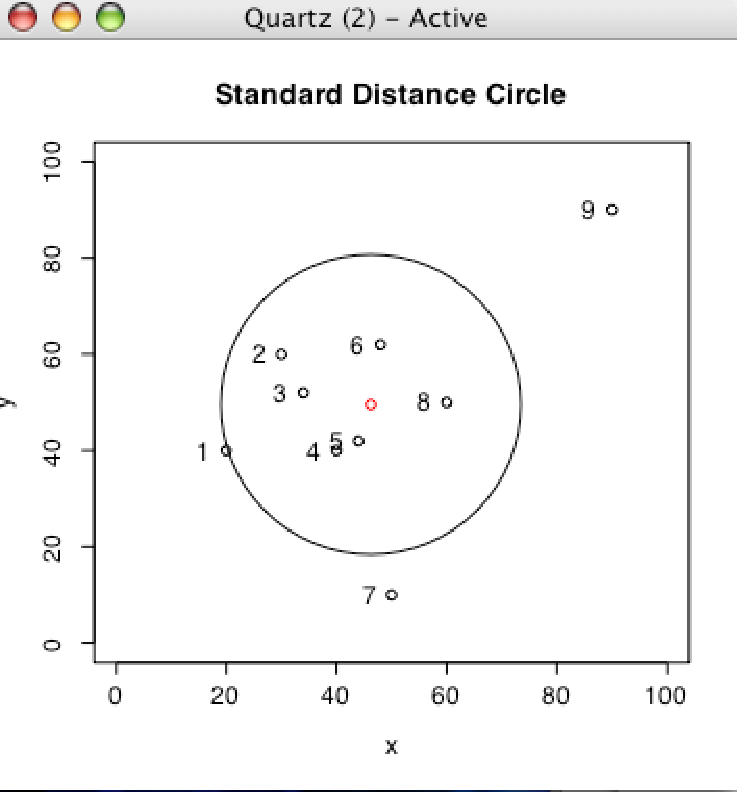
\includegraphics[width=.65\linewidth]{standardDistance1}
   \end{center}
 \end{frame}

 \begin{frame}
   \frametitle{Standard Deviational Ellipse}
   \begin{block}{Relative to Standard Distance}
     \begin{itemize}
       \item Measures dispersion
       \item Sensitive to \emph{shape} of distribution
       \item Measures dispersion in two dimensions
     \end{itemize}
    \end{block}
    \begin{block}{Components}
      \begin{itemize}
	\item Angle of rotation
	\item Dispersion along major axis
	\item Dispersion along minor axis
      \end{itemize}
     \end{block}
  \end{frame}

 \begin{frame}
   \frametitle{Standard Deviational Ellipse}
   \begin{block}{Major, minor axes}
     \begin{itemize}
       \item Major axis defines the direction of maximum spread in the
	 distribution
       \item Minor axis is orthogonal to major axis
       \item Minor axis defines the direction of minimum spread
     \end{itemize}
    \end{block}
    \begin{block}{Steps}
      \begin{enumerate}
	\item Determine rotation angle of $Y$-axis
	\item Calculate standard deviations for transposed axes
	\item Determine length of axes
	\item Determine area of the ellipse
      \end{enumerate}
     \end{block}
 \end{frame}
\begin{frame}
   \frametitle{Rotation Angle $\Theta$}
   \begin{block}{}
     \begin{eqnarray*}
       \Theta = ARCTAN \left\{ \left( \sum_{i} (x_i-\bar{x})^2  -\sum_{i} (y_i-\bar{y})^2  \right) + \right. \\
     \left[ \left( \sum_{i} (x_i-\bar{x})^2  -\sum_{i} (y_i-\bar{y})^2 \right)^2  + \right. \\
  	\left .\left.  4\left(  \sum_{i} (x_i-\bar{x}) (y_i-\bar{y})\right)^2
	\right]^{1/2} \right\} / \\
 2\sum_{i} (x_i-\bar{x}) (y_i-\bar{y})
  \end{eqnarray*}
    \end{block}
 \end{frame}

 \begin{frame}
   \frametitle{Standard Deviations On Transposed Axes}
   \begin{block}{$S_x$}
     \begin{equation}
       S_x = \sqrt{ 2\frac{(\sum_{i=1}^n (x_i-\bar{x})Cos(\Theta) -
       \sum_{i=1}^n (y_i-\bar{y})Sin(\Theta))^2}{n-2}}
     \end{equation}
    \end{block}
\begin{block}{$S_y$}
     \begin{equation}
       S_y = \sqrt{ 2\frac{(\sum_{i=1}^n (x_i-\bar{x})Sin(\Theta) -
       \sum_{i=1}^n (y_i-\bar{y})Cos(\Theta))^2}{n-2}}
     \end{equation}
    \end{block}

  \end{frame}

  \begin{frame}
    \frametitle{Ellipse Axes}
    \begin{block}{Lengths}
      \begin{equation}
	L_x = 2 S_x
      \end{equation}
      \begin{equation}
	L_y = 2 S_y
      \end{equation}
     \end{block}
     \begin{block}{Mid Point}
	Mean Center of Point Pattern $(x_m,y_m)$
     \end{block}
     \begin{block}{Area}
       \begin{equation}
       A = \pi S_x S_y
       \end{equation}
     \end{block}


   \end{frame}

\begin{frame}
   \frametitle{Standard Deviational Ellipse}
   \begin{center}
     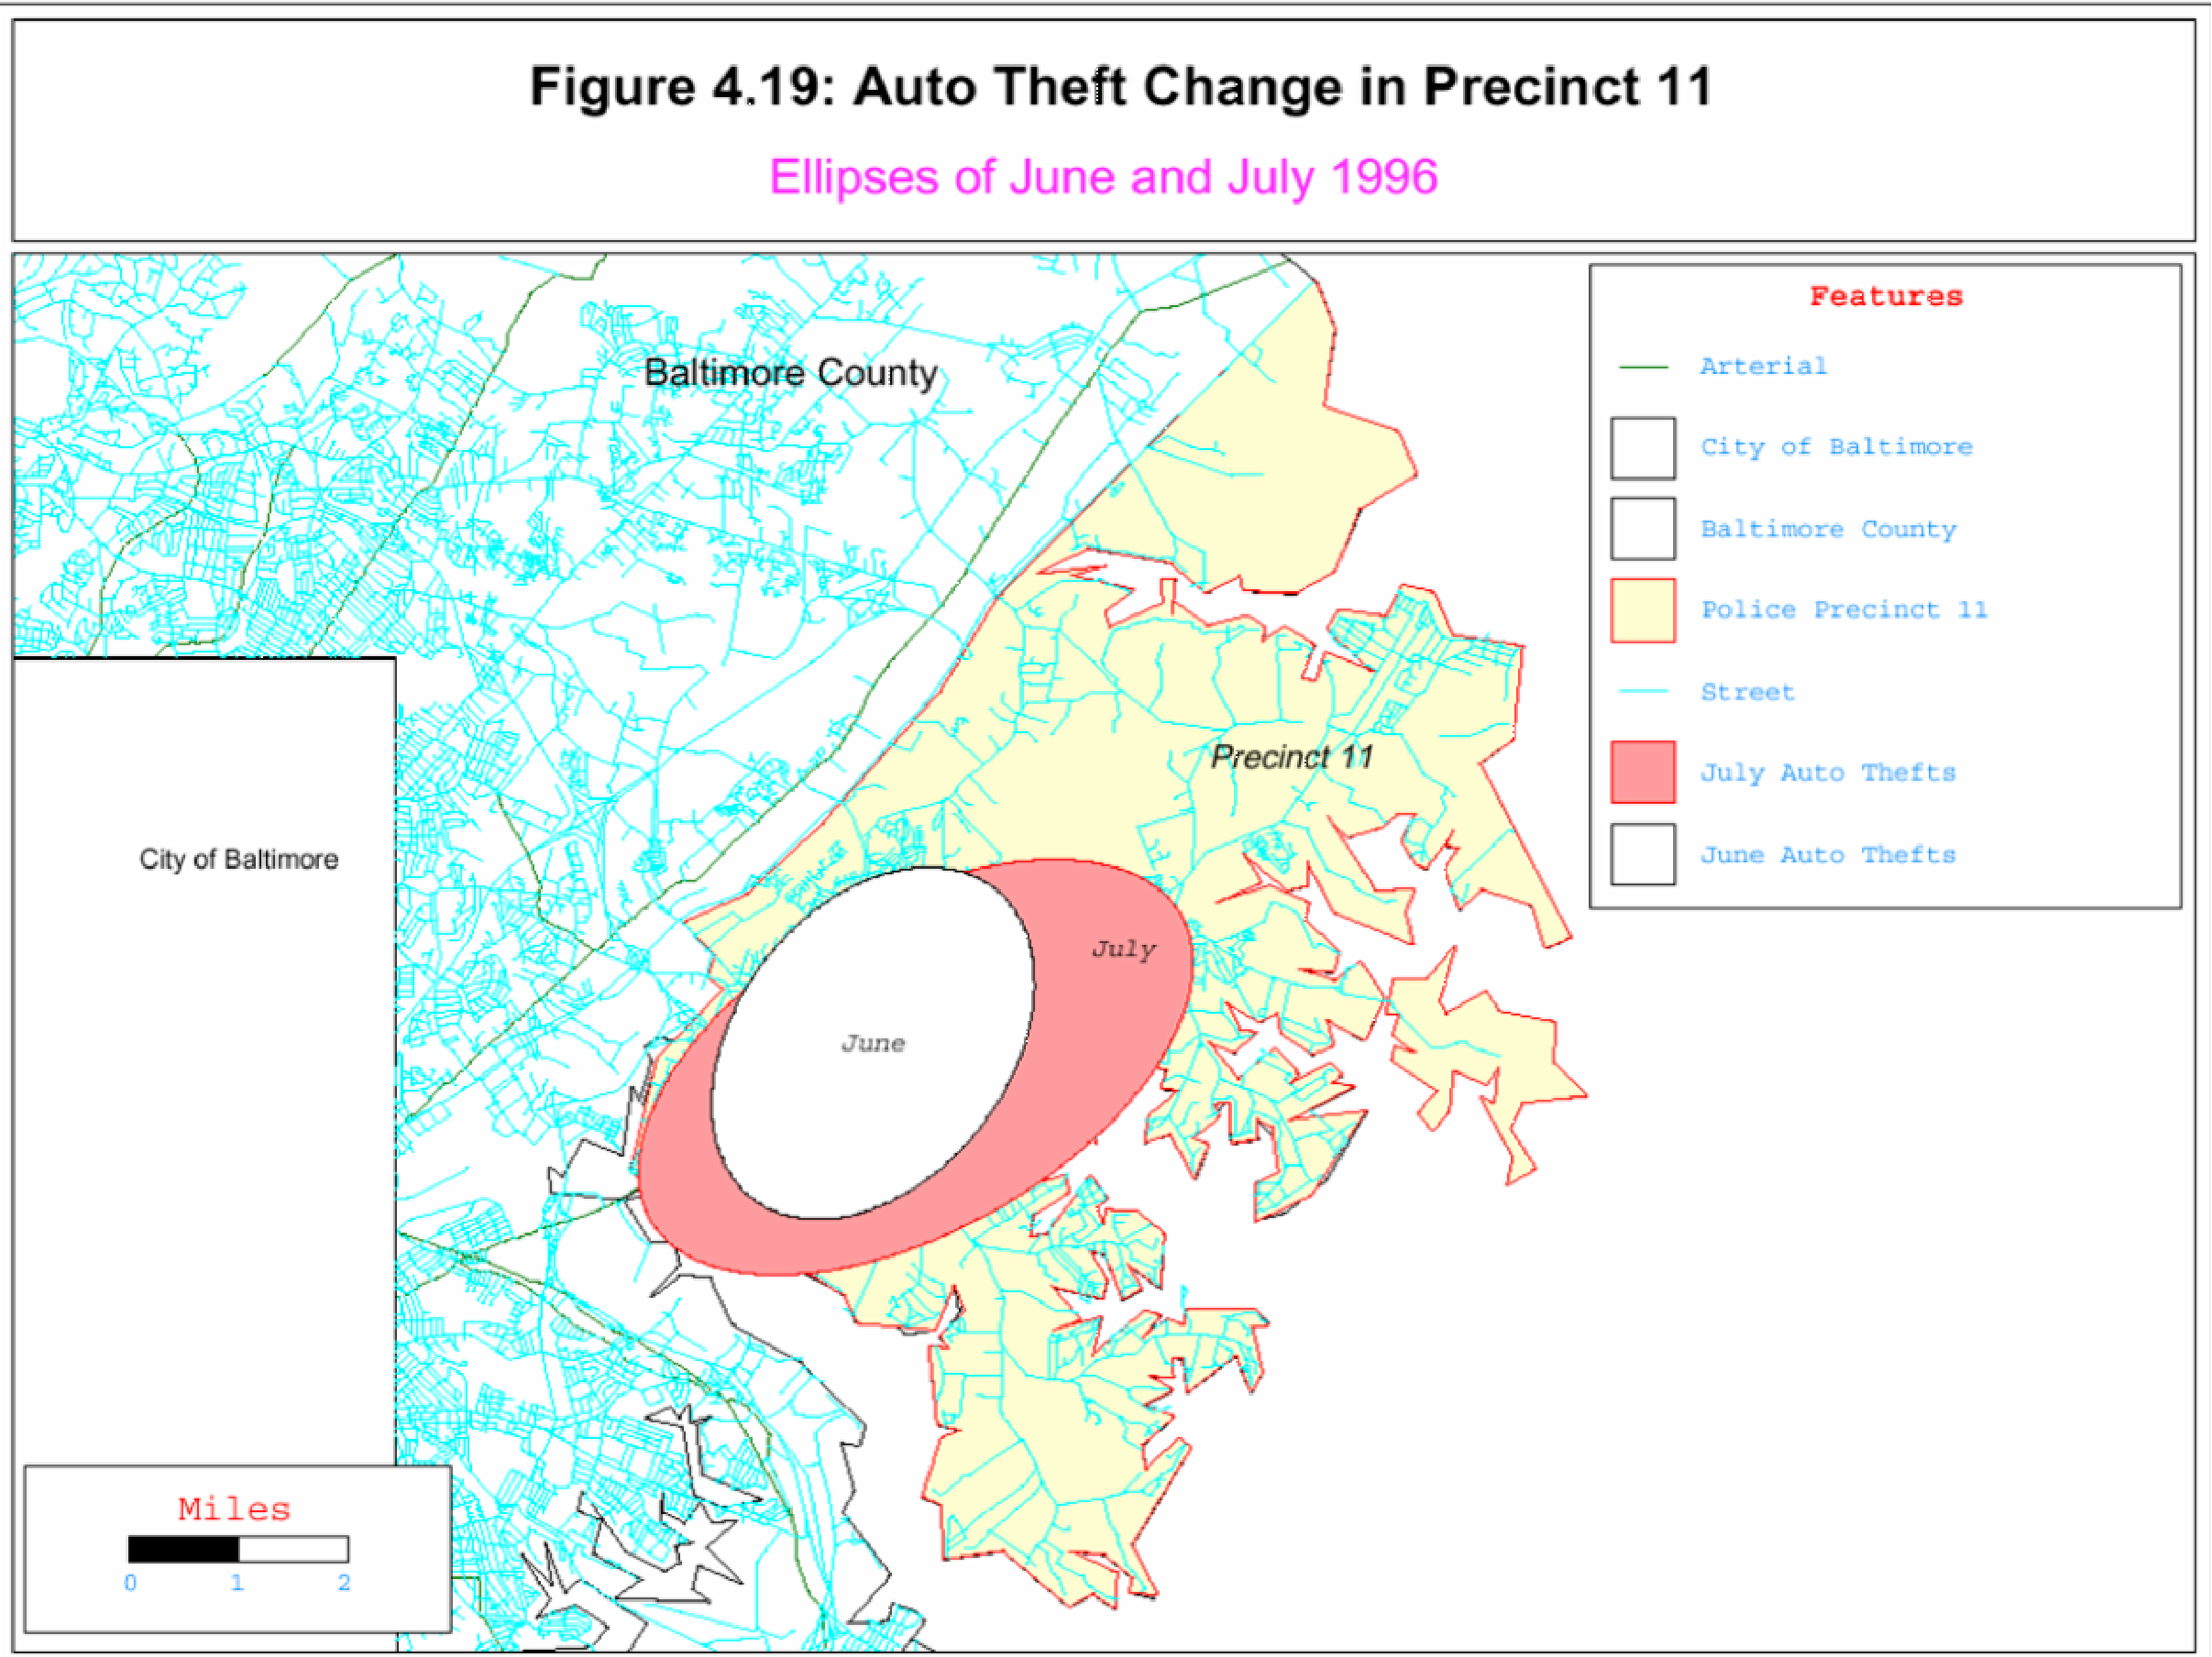
\includegraphics[width=.85\linewidth]{ellipse}
   \end{center}
 \end{frame}



\subsection{Geometry}
\begin{frame}
  \frametitle{Shape Analysis of Point Patterns}
  \begin{block}{Geometry}
    \begin{itemize}
      \item Bounding Box
      \item Convex Hulls
    \end{itemize}
   \end{block}
 \end{frame}

\begin{frame}
   \frametitle{Bounding Box}
   \begin{center}
     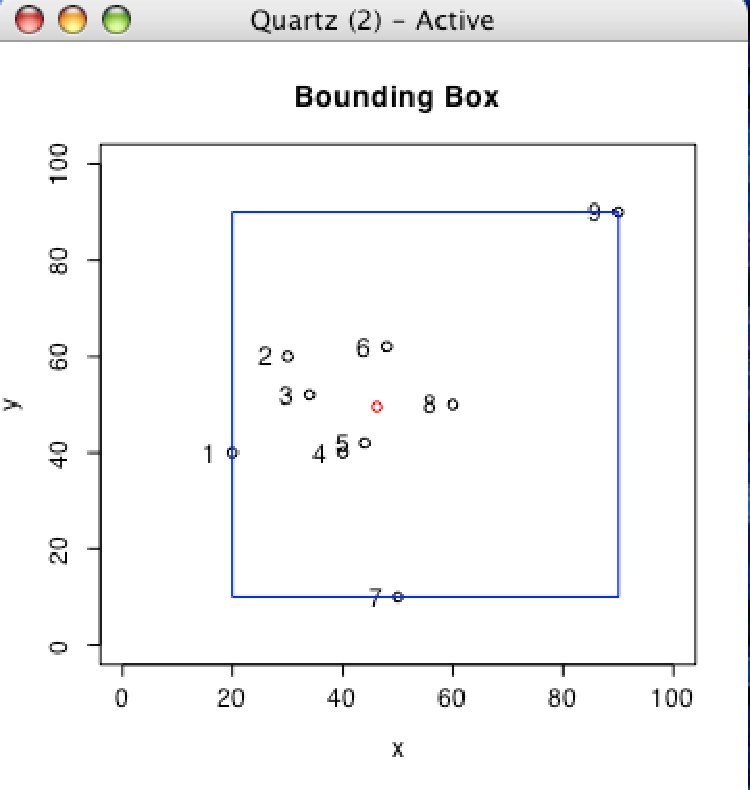
\includegraphics[width=.65\linewidth]{ppbbox}
   \end{center}
 \end{frame}

\begin{frame}
   \frametitle{Convex Hull}
   \begin{center}
     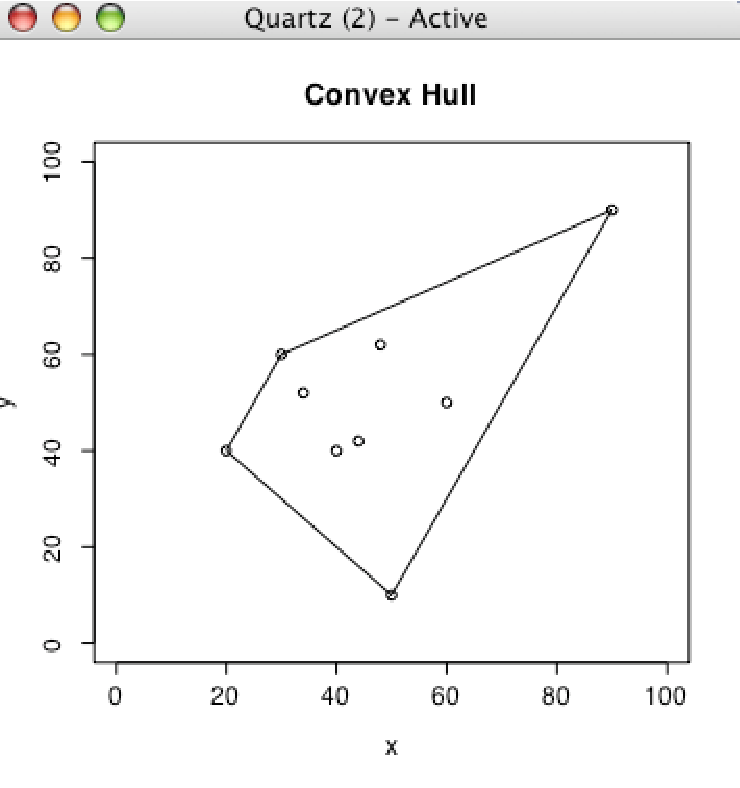
\includegraphics[width=.65\linewidth]{ppconvex}
   \end{center}
 \end{frame}

\begin{frame}
   \frametitle{Convex Hull and Bounding Box}
   \begin{center}
     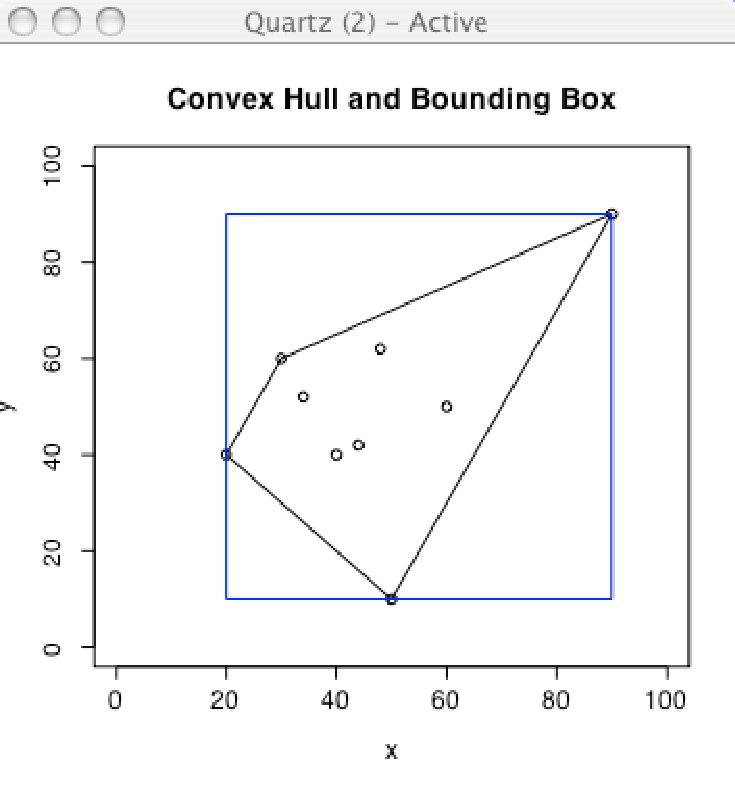
\includegraphics[width=.65\linewidth]{ppbbconvex}
   \end{center}
 \end{frame}

\begin{frame}
   \frametitle{Convex Hull (Large n)}
   \begin{center}
     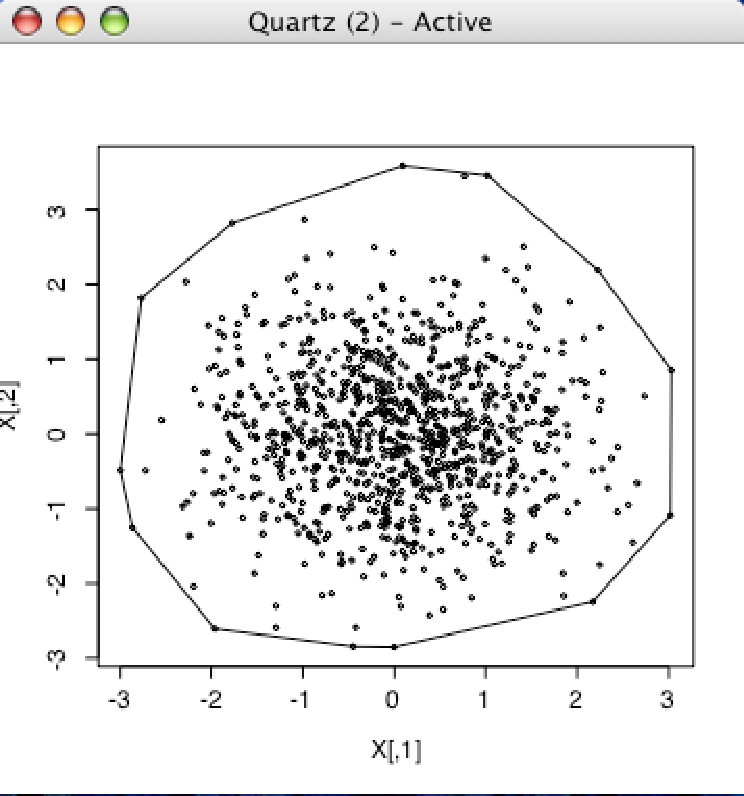
\includegraphics[width=.65\linewidth]{ppconvex1}
   \end{center}
 \end{frame}

\begin{frame}
   \frametitle{Nested Convex Hulls}
   \begin{center}
     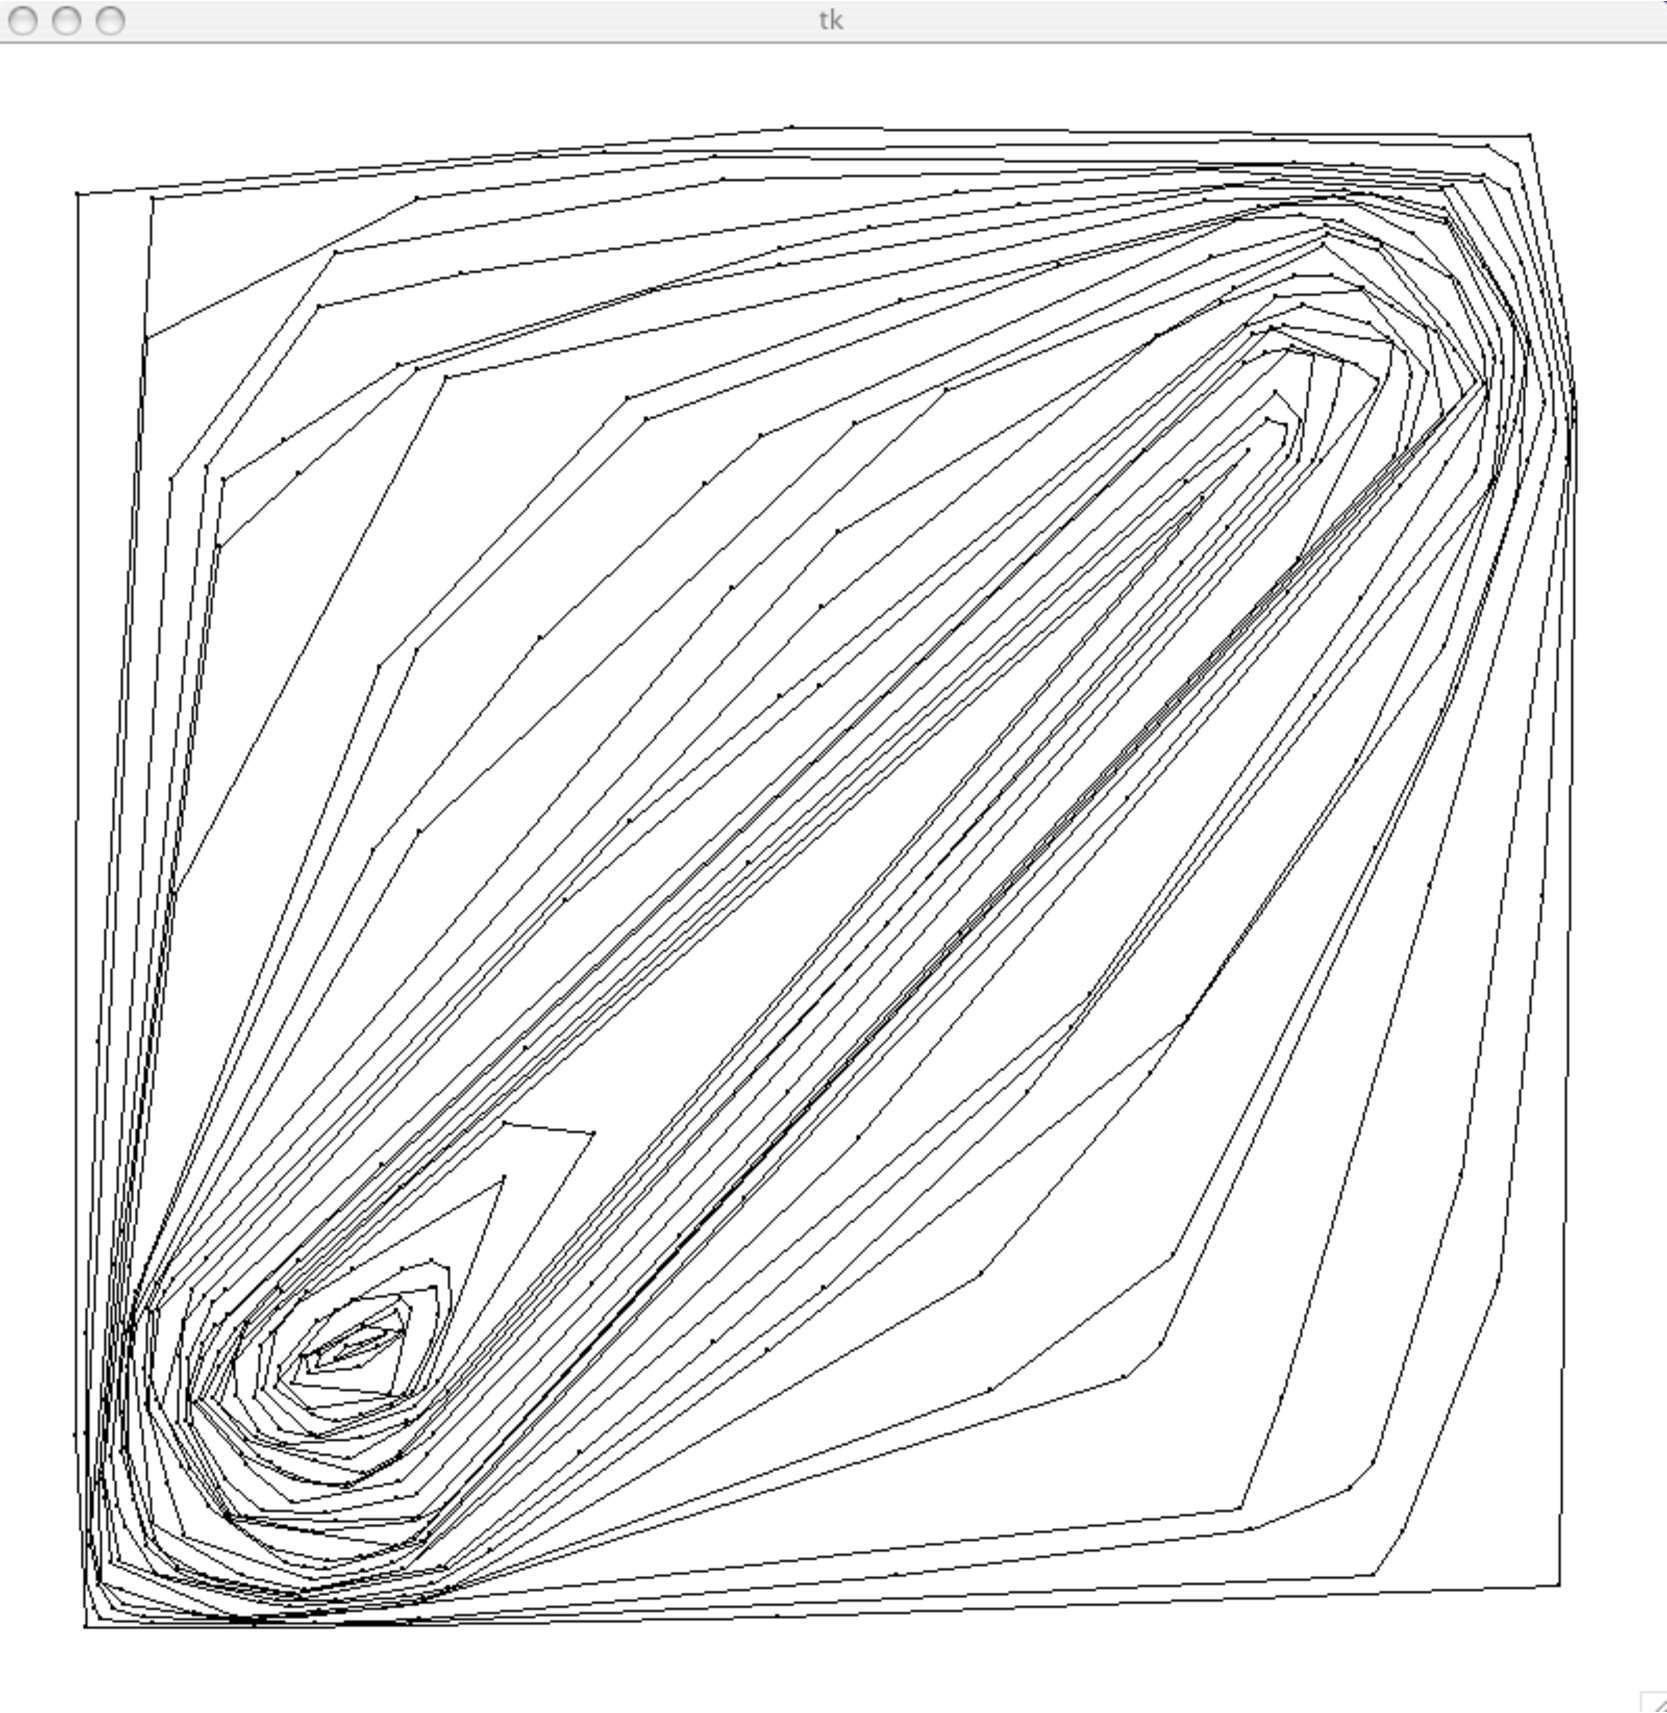
\includegraphics[width=.65\linewidth]{nestedHulls}
   \end{center}
 \end{frame}



\section{Kernel Density Estimation}

\end{document}
